\chapter{Deep learning} 
\section{Introduction}
    Deep learning is a type of Machine learning(ML) that has a goal to imitate the human approach to learning
    certain tasks \cite{Deep learning}. 

    At its core, deep learning is a way to automate predictive analytics on certain data sets, in our case X-Ray images of lungs.
    This automation of predictive analytics is base for the main difference between traditional AI and deep learning, where AI algorithm 
    is linear in its nature, and deep learning algorithms are using the method of stacking layers upon each other, each layer has an increasing 
    complexity and abstraction. By this hierarchical approach, we are able to create abstract layers based on the knowledge from the previous layer.
    %A prime example of this hierarchy is Convolutional Neural Network (CNN), which uses multiple different layers to deliver the desired output. 
    %\begin{figure} 
        %\centering
        %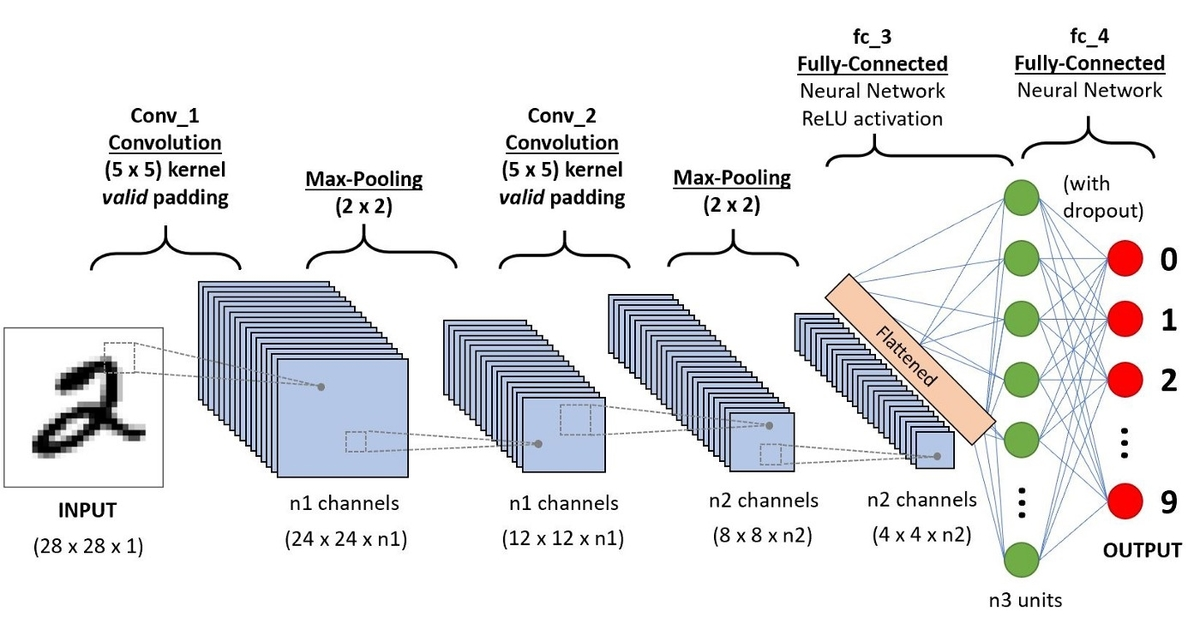
\includegraphics[width=.75\textwidth]{pict/CNN_Architecture.jpg}
        %\caption{basic CNN architecture}
    %\end{figure}

\section{Capsule Neural Network}
    \subsection{Description}
        Capsule Neural Network (Caps Net) represents the latest breakthrough in the field of neural networks architecture. 
        This new architecture is able to achieve better results on Modified National Institute of Standards and Technology database than conventional CNN. 
        Error results on this dataset were set to be 0.39\% 
        until Caps Net was introduced which achieved a score of 0.25\% without any data augmentation \cite{Capsule Neural Network performance on complex data}. 
        To achieve such performance Caps Net uses  concept of capsules as proposed by Hinton \cite{Dynamic routing between capsules}. By this method each
        capsule creates its own output, by combining outputs from all the capsules we are able to create much more stable and precise output.

        Caps Net was created and proposed to address two big issues that were introduced with the usage of CNN, which saw an increase in application in recent years. 
        CNN's failure to account for spatial hierarchies between features and lack rotational invariance \cite{Dynamic routing between capsules}. 
        Since CNN classifies the test data as the object and disregards any spatial relative features, this approach causes an increase in false positive cases. 
        The second issue is lack of rotational invariance causing the network to assign an incorrect label to the object increasing false negative cases. 

        Earlier in this section, we have stated the reasons that brought to life Caps Net architecture. That being said, let's turn our attention to the history of Caps Net. 
        The first predecessor of Caps Net was proposed by Geoffrey Hinton in 2000. In the paper named Learning to Parse Images \cite{Learning To Parse Images}, in this paper, Hinton described a new imaging system that would use a combination of segmentation and recognition. 
        This combination would then be put into a single interface process using the parse tree. 
        In the year 2011, Hinton published a second paper expanding on this very basic idea of the parse tree \cite{Transforming Auto-Encoders}. 
        In this paper, he introduced the concept of the capsules to CNN architecture. 
        The basic idea is that we add these capsule structures to CNN and use the output from several of those capsules to form a more stable representation of higher capsules. 
        This will create an output vector that can be further processed.  After this paper, Hinton and his team published a third paper on the topic of Caps Net \cite{Dynamic routing between capsules}. In this paper, Hinton and his team proposed the utilization of dynamic routing between capsules. 
        As stated in the paper, there are many ways to implement capsule architecture, but not all of them are as straightforward as proposed by Hinton. 
        This approach is further supported by the utilization of dynamic routing. 
    \subsection{Architecture}\
    \subsection{Benefits and downsides of Caps Net over CNN}
    \subsection{Real world application of Capsulated Neural Network}

\section{Residual Neural Network}
    \subsection{Description}
    \subsection{Architecture}
    \subsection{Real world application of Residual Network}

\section{Medical application}
